\chapter{光照基础}
\minitoc


我与Cocos2d-x结缘于2011年,那个时候我所在的公司OpenXLive与Cocos2d-x团队合作移植Cocos2d-x游戏引擎到WP7平台,它采用C\#语言基于XNA来实现,我成为该项目的负责人。然而不久微软就用支持C++原生语言的WP8替代了WP7,该项目也逐渐被开发者淡忘。然而不想三年后我却会为Cocos2d-x写一本书,这三年,我和Cocos2d-x都在成长~\cite{test}。


开源,是我认为软件最富魅力的部分,它给予我们阅读和修改源代码的自由。开源对人类和科技进步的贡献是巨大的,如今,几乎大多数软件系统都有着各种各样开源软件的影子。另一方面,开源代码对技术人员的成长有着难以估量的价值,例如,没有开源的Cocos2d-x,我就难以写出本书中的很多内容。

本书定位为一本进阶的书籍,它着重于讲述Cocos2d-x引擎各个功能及组件背后的实现原理。因此,本书并没有严格按照Cocos2d-x引擎本身的功能展开描述,而是从这些功能中抽象出一些设计或者架构层面的内容进行讨论。例如本书没有分别讲述精灵,地图,粒子特效等的接口使用,而是从纹理,渲染方式等多个方面来讲述这些元素背后的工作机制;而OpenGL ES,物理引擎和脚本等内容也几乎是可以脱离于Cocos2d-x进行学习和理解的。

这就是本书标题的来源,也是本书与同类书籍在内容编排上的最大不同。我希望写作一本书,它可以让读者站在一个系统性的高度对游戏引擎的一些架构设计及实现进行理解,从而不但提升和扩充自己的知识结构,更能够在实际开发中去灵活解决各个层面的技术问题。另外,本书同时也追求系统性和实践性的一个平衡,例如对于纹理部分,除了总结了纹理相关的所有知识,也通过一些示例来演示它在各个层面的具体使用。

本书一共分十八的章节,第1-4章介绍了Cocos2d-x引擎的基本架构以及新的绘制系统。这部分包括Cocos2d-x的内存管理机制,UI树的遍历及结构,应用程序的生命周期,游戏循环的各个阶段以及在Cocos2d-x中驱动各个子系统进行逻辑更新的机制及工作原理。这部分也介绍了3.x新的数据结构,以及详细描述了新的渲染系统。总之,在这一部分,读者可以对Cocos2d-x的基本架构有一些比较系统的了解。

第5-10章围绕OpenGL ES图形渲染管线进行介绍。这部分从纹理讲起,详细讲述了纹理的存储格式,传输,缩放,压缩以及多重纹理等相关知识;第8章详细讲述了顶点数组的结构,顶点属性的绑定及传输,着色器程序的编译及链接;以及Cocos2d-x新的着色器子系统,并举例在Cocos2d-x中使用着色器的流程以及怎样使用多重纹理。这部分也对顶点着色器和片段着色器两个阶段在图形渲染管线中的作用进行了详细描述。

\begin{fullwidth}
第9,10章讲述OpenGL ES图形渲染管线的最后两个阶段:帧缓冲和片段操作,并以Cocos2d-x中对这两个阶段的应用RenderTexture和ClippingNode为例进行讲解。这样,读者将对整个渲染管线的每一个阶段都能有所了解,并且能够结合Cocos2d-x中的使用去思考每一个阶段的意义和作用,从而对图形渲染管线有更深刻的了解。这也是本书最具特色的部分。
\end{fullwidth}


第10-15章讲述Cocos2d-x的一些子系统,包括事件分发,多分辨率支持,动画系统以及物理引擎整合。其中物理引擎部分也是我比较喜欢的章节,这部分讲述了一些通用的物理引擎的架构,使用以及怎样和游戏引擎进行整合。

第16-18章探讨应该怎样去设计和管理游戏世界中的对象。16章首先讲述了常见对象模型,组件模型以及属性模型之间的一些概念,区别以及优缺点;第17章则以属性模型为例讲述了一个游戏对象模型应该怎样设计;第18章探讨了时下最流行的脚本相关的内容,但是与仅仅讨论脚本使用不同的是,我们站在一个游戏引擎的高度,去讨论脚本的架构,这样读者甚至能设计自己的脚本模型。这一部分的内容,具有对前端架构设计的高度总结性与实践性,不管是对经验丰富的读者还是初学者,相信都具有一定的启发性。

另外,这本书在写作之初并没有构建出整本书的内容结构,在写前面的章节时我甚至不知道最后几章的内容和结构会是怎样的。在开始写每一章的时候,我不会首先去给自己描绘一个目录结构,而是首先去把所有相关的内容列出来,如果之中有我不熟悉的内容,或者有Cocos2d-x以外的一些知识,则我会首先停下写作去把这些内容整理出来。例如关于ECS部分的内容就是基于Cocos2d-x社区的一些讨论,然后花了很多时间去学习和理解。当最后所有相关的内容整理为一个列表时,我就知道该怎么去写作这部分的内容。因此,在这本书的目录结构中,你找不到任何同类书籍类似的内容结构,因为这完全是基于个人的理解及知识结构体系去写作的一本书。

\begin{fullwidth}
	

所以,对我而言这本书还有一个有意义的目标,我希望透过这样的方式去探讨一种系统性的学习方法,当你开始学习某个知识点时,不要把自己限定在该知识点处,而是首先从该知识点进行适当的扩展,列出该知识点相关的所有内容,然后再逐个深入学习和研究细节,最后反过来整理该知识点的结构体系。这样不仅能够更深入地学习该知识点,还能够延伸知识的广度,所以本书有大量超出Cocos2d-x以外的内容,这些内容又是与Cocos2d-x紧密相关的。希望读者在阅读过程中能够感受到这样一种写作风格和方法。

\end{fullwidth}

本书是一本进阶类书籍,阅读本书,你需要对Cocos2d-x和C++有一些基本的了解。如果你是一个新手,可以首先阅读一些同类书籍中相对比较入门的书籍,否则本书的一些章节可能会给你造成一定的困惑。

学习知识最好的方法永远是多读几面,书中比如关于OpenGL ES和游戏对象模型部分的内容可能需要多读几次才能更加深入地理解相关的概念。当然,如果你在阅读过程中遇到什么障碍,随时可以通过电子邮件或者我的博客等多种方式和我进行探讨。

本书可以作为Cocos2d-x开发学习的书籍,也可以作为单独的OpenGL ES相关的教材,游戏对象模型部分的内容也可以作为设计游戏引擎架构的参考资料。本书也可以作为高校游戏及图形学相关专业的参考教程。

最后,由于个人经验有限,思维有限,所以书中难免出现一些错误。真诚地希望读者可以将这些错误的地方反馈给出版社,我们会及时地列出勘误,以帮助更多的读者更好地学习。


\begin{figure}
\begin{fullwidth}
	\begin{subfigure}[b]{0.33\thewidth}
		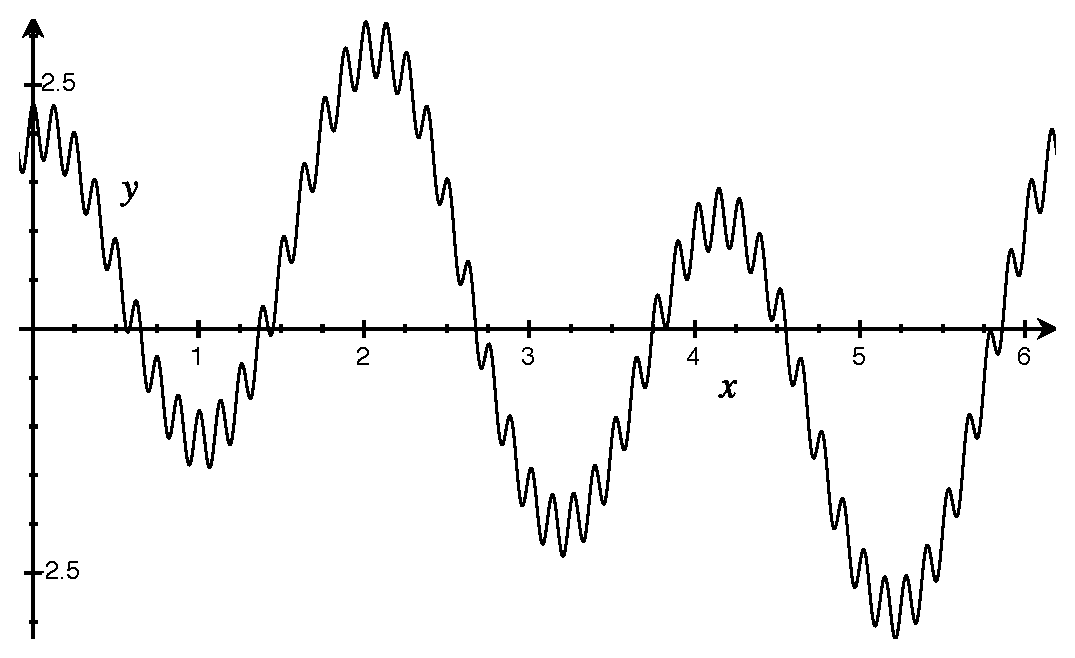
\includegraphics[width=1.\textwidth]{figures/intro/fourier-1}
	\end{subfigure}
	\begin{subfigure}[b]{0.33\thewidth}
		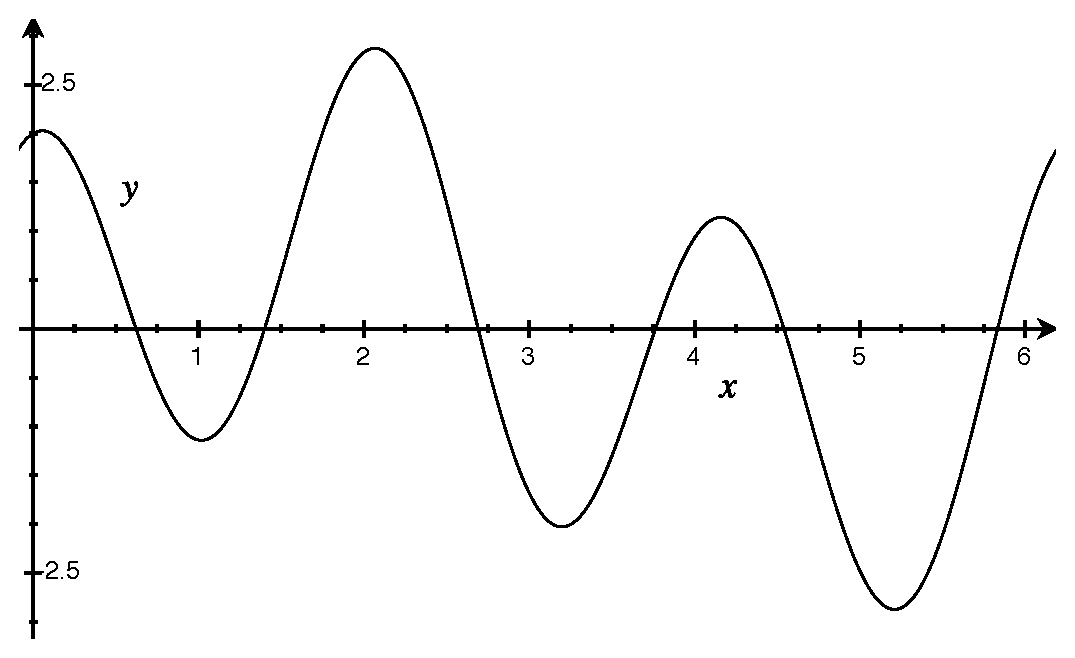
\includegraphics[width=1.\textwidth]{figures/intro/fourier-2}
	\end{subfigure}
	\begin{subfigure}[b]{0.33\thewidth}
		\includegraphics[width=1.\textwidth]{figures/intro/fourier-3}
	\end{subfigure}
\caption{傅立叶变换将函数由时间域(或空间域)变换到频率域(图片来自Wikipedia)。}
\label{f:intro-fourier}
\end{fullwidth}
\end{figure}


\abstract*{Each chapter should be preceded by an abstract (10--15 lines long) that summarizes the content. The abstract will appear \textit{online} at \url{www.SpringerLink.com} and be available with unrestricted access. This allows unregistered users to read the abstract as a teaser for the complete chapter. As a general rule the abstracts will not appear in the printed version of your book unless it is the style of your particular book or that of the series to which your book belongs.
Please use the 'starred' version of the new Springer \texttt{abstract} command for typesetting the text of the online abstracts (cf. source file of this chapter template \texttt{abstract}) and include them with the source files of your manuscript. Use the plain \texttt{abstract} command if the abstract is also to appear in the printed version of the book.}


\section{Section Heading}
Use the template \emph{chapter.tex} together with the Springer document class SVMono (monograph-type books) or SVMult (edited books) to style the various elements of your chapter content in the Springer layout.

\section{Section Heading}
\label{sec:2}
% Always give a unique label
% and use \ref{<label>} for cross-references
% and \cite{<label>} for bibliographic references
% use \sectionmark{}
% to alter or adjust the section heading in the running head
Instead of simply listing headings of different levels we recommend to let every heading be followed by at least a short passage of text. Furtheron please use the \LaTeX\ automatism for all your cross-references and citations.

Please note that the first line of text that follows a heading is not indented, whereas the first lines of all subsequent paragraphs are.

Use the standard \verb|equation| environment to typeset your equations, e.g.
%
\begin{equation}
a \times b = c\;,
\end{equation}
%
however, for multiline equations we recommend to use the \verb|eqnarray|
environment\footnote{In physics texts please activate the class option \texttt{vecphys} to depict your vectors in \textbf{\itshape boldface-italic} type - as is customary for a wide range of physical subjects.}.
\begin{eqnarray}
a \times b = c \nonumber\\
\vec{a} \cdot \vec{b}=\vec{c}
\label{eq:01}
\end{eqnarray}

\subsection{Subsection Heading}
\label{subsec:2}
Instead of simply listing headings of different levels we recommend to let every heading be followed by at least a short passage of text. Furtheron please use the \LaTeX\ automatism for all your cross-references\index{cross-references} and citations\index{citations} as has already been described in Sect.~\ref{sec:2}.

\begin{quotation}
Please do not use quotation marks when quoting texts! Simply use the \verb|quotation| environment -- it will automatically render Springer's preferred layout.
\end{quotation}


\subsubsection{Subsubsection Heading}
Instead of simply listing headings of different levels we recommend to let every heading be followed by at least a short passage of text. Furtheron please use the \LaTeX\ automatism for all your cross-references and citations as has already been described in Sect.~\ref{subsec:2}, see also Fig.~\ref{fig:1}\footnote{If you copy text passages, figures, or tables from other works, you must obtain \textit{permission} from the copyright holder (usually the original publisher). Please enclose the signed permission with the manucript. The sources\index{permission to print} must be acknowledged either in the captions, as footnotes or in a separate section of the book.}

Please note that the first line of text that follows a heading is not indented, whereas the first lines of all subsequent paragraphs are.

% For figures use
%

	

\begin{figure}[b]

%\sidecaption
% Use the relevant command for your figure-insertion program
% to insert the figure file.
% For example, with the option graphics use
\includegraphics[scale=.65]{figure}
%
% If not, use
%\picplace{5cm}{2cm} % Give the correct figure height and width in cm
%
\caption{If the width of the figure is less than 7.8 cm use the \texttt{sidecapion} command to flush the caption on the left side of the page. If the figure is positioned at the top of the page, align the sidecaption with the top of the figure -- to achieve this you simply need to use the optional argument \texttt{[t]} with the \texttt{sidecaption} command}
\label{fig:12}       % Give a unique label

\end{figure}



\paragraph{Paragraph Heading} %
Instead of simply listing headings of different levels we recommend to let every heading be followed by at least a short passage of text. Furtheron please use the \LaTeX\ automatism for all your cross-references and citations as has already been described in Sect.~\ref{sec:2}.

Please note that the first line of text that follows a heading is not indented, whereas the first lines of all subsequent paragraphs are.

For typesetting numbered lists we recommend to use the \verb|enumerate| environment -- it will automatically render Springer's preferred layout.

\begin{figure}[b]
\sidecaption
% Use the relevant command for your figure-insertion program
% to insert the figure file.
% For example, with the option graphics use
\includegraphics[scale=.65]{figure}
%
% If not, use
%\picplace{5cm}{2cm} % Give the correct figure height and width in cm
%
\caption{If the width of the figure is less than 7.8 cm use the \texttt{sidecapion} command to flush the caption on the left side of the page. If the figure is positioned at the top of the page, align the sidecaption with the top of the figure -- to achieve this you simply need to use the optional argument \texttt{[t]} with the \texttt{sidecaption} command}
\label{fig:19}       % Give a unique label
\end{figure}

\begin{enumerate}
\item{Livelihood and survival mobility are oftentimes coutcomes of uneven socioeconomic development.}
\begin{enumerate}
\item{Livelihood and survival mobility are oftentimes coutcomes of uneven socioeconomic development.}
\item{Livelihood and survival mobility are oftentimes coutcomes of uneven socioeconomic development.}
\end{enumerate}
\item{Livelihood and survival mobility are oftentimes coutcomes of uneven socioeconomic development.}
\end{enumerate}


\subparagraph{Subparagraph Heading} In order to avoid simply listing headings of different levels we recommend to let every heading be followed by at least a short passage of text. Use the \LaTeX\ automatism for all your cross-references and citations as has already been described in Sect.~\ref{sec:2}, see also Fig.~\ref{fig:2}.

Please note that the first line of text that follows a heading is not indented, whereas the first lines of all subsequent paragraphs are.

For unnumbered list we recommend to use the \verb|itemize| environment -- it will automatically render Springer's preferred layout.

\begin{itemize}
\item{Livelihood and survival mobility are oftentimes coutcomes of uneven socioeconomic development, cf. Table~\ref{tab:1}.}
\begin{itemize}
\item{Livelihood and survival mobility are oftentimes coutcomes of uneven socioeconomic development.}
\item{Livelihood and survival mobility are oftentimes coutcomes of uneven socioeconomic development.}
\end{itemize}
\item{Livelihood and survival mobility are oftentimes coutcomes of uneven socioeconomic development.}
\end{itemize}

\begin{figure}[t]
\sidecaption[t]
% Use the relevant command for your figure-insertion program
% to insert the figure file.
% For example, with the option graphics use
\includegraphics[scale=.65]{figure}
%
% If not, use
%\picplace{5cm}{2cm} % Give the correct figure height and width in cm
%
\caption{Please write your figure caption here}
\label{fig:2}       % Give a unique label
\end{figure}

\runinhead{Run-in Heading Boldface Version} Use the \LaTeX\ automatism for all your cross-references and citations as has already been described in Sect.~\ref{sec:2}.

\subruninhead{Run-in Heading Italic Version} Use the \LaTeX\ automatism for all your cross-refer\-ences and citations as has already been described in Sect.~\ref{sec:2}\index{paragraph}.
% Use the \index{} command to code your index words
%
% For tables use
%


	
		

\begin{table}

\caption{Please write your table caption here. Please write your table caption here. Please write your table caption here}
\label{tab:1}       % Give a unique label
%
% For LaTeX tables use
%
\begin{tabular}{p{3cm}p{3.4cm}p{3cm}p{4.9cm}}
\hline\noalign{\smallskip}
Classes & Subclass & Length & Action Mechanism  \\
\noalign{\smallskip}\svhline\noalign{\smallskip}
Translation & mRNA$^a$  & 22 (19--25) & Translation repression, mRNA cleavage\\
Translation & mRNA cleavage & 21 & mRNA cleavage\\
Translation & mRNA  & 21--22 & mRNA cleavage\\
Translation & mRNA  & 24--26 & Histone and DNA Modification\\
\noalign{\smallskip}\hline\noalign{\smallskip}
\end{tabular}
\end{table}
	



%
\section{Section Heading}
\label{sec:3}
% Always give a unique label
% and use \ref{<label>} for cross-references
% and \cite{<label>} for bibliographic references
% use \sectionmark{}
% to alter or adjust the section heading in the running head
Instead of simply listing headings of different levels we recommend to let every heading be followed by at least a short passage of text. Furtheron please use the \LaTeX\ automatism for all your cross-references and citations as has already been described in Sect.~\ref{sec:2}.

Please note that the first line of text that follows a heading is not indented, whereas the first lines of all subsequent paragraphs are.

If you want to list definitions or the like we recommend to use the Springer-enhanced \verb|description| environment -- it will automatically render Springer's preferred layout.

\begin{description}[Type 1]
\item[Type 1]{That addresses central themes pertainng to migration, health, and disease. In Sect.~\ref{sec:1}, Wilson discusses the role of human migration in infectious disease distributions and patterns.}
\item[Type 2]{That addresses central themes pertainng to migration, health, and disease. In Sect.~\ref{subsec:2}, Wilson discusses the role of human migration in infectious disease distributions and patterns.}
\end{description}

\subsection{Subsection Heading} %
In order to avoid simply listing headings of different levels we recommend to let every heading be followed by at least a short passage of text. Use the \LaTeX\ automatism for all your cross-references and citations citations as has already been described in Sect.~\ref{sec:2}.

Please note that the first line of text that follows a heading is not indented, whereas the first lines of all subsequent paragraphs are.

\begin{svgraybox}
If you want to emphasize complete paragraphs of texts we recommend to use the newly defined Springer class option \verb|graybox| and the newly defined environment \verb|svgraybox|. This will produce a 15 percent screened box 'behind' your text.

If you want to emphasize complete paragraphs of texts we recommend to use the newly defined Springer class option and environment \verb|svgraybox|. This will produce a 15 percent screened box 'behind' your text.
\end{svgraybox}


\subsubsection{Subsubsection Heading}
Instead of simply listing headings of different levels we recommend to let every heading be followed by at least a short passage of text. Furtheron please use the \LaTeX\ automatism for all your cross-references and citations as has already been described in Sect.~\ref{sec:2}.

Please note that the first line of text that follows a heading is not indented, whereas the first lines of all subsequent paragraphs are.

\begin{theorem}
Theorem text goes here.
\end{theorem}
%
% or
%
\begin{definition}
Definition text goes here.
\end{definition}

\begin{proof}
%\smartqed
Proof text goes here.
\qed
\end{proof}

\paragraph{Paragraph Heading} %
Instead of simply listing headings of different levels we recommend to let every heading be followed by at least a short passage of text. Furtheron please use the \LaTeX\ automatism for all your cross-references and citations as has already been described in Sect.~\ref{sec:2}.

Note that the first line of text that follows a heading is not indented, whereas the first lines of all subsequent paragraphs are.
%
% For built-in environments use
%
\begin{theorem}
Theorem text goes here.
\end{theorem}
%
\begin{definition}
Definition text goes here.
\end{definition}
%
\begin{proof}
\smartqed
Proof text goes here.
\qed
\end{proof}
%
\begin{acknowledgement}
If you want to include acknowledgments of assistance and the like at the end of an individual chapter please use the \verb|acknowledgement| environment -- it will automatically render Springer's preferred layout.
\end{acknowledgement}
%
\section{Appendix}
%
When placed at the end of a chapter or contribution (as opposed to at the end of the book), the numbering of tables, figures, and equations in the appendix section continues on from that in the main text. Hence please \textit{do not} use the \verb|appendix| command when writing an appendix at the end of your chapter or contribution. If there is only one the appendix is designated ``Appendix'', or ``Appendix 1'', or ``Appendix 2'', etc. if there is more than one.

\begin{equation}
a \times b = c
\end{equation}
% Problems or Exercises should be sorted chapterwise
\section{Problems}
\addcontentsline{toc}{section}{Problems}
%
% Use the following environment.
% Don't forget to label each problem;
% the label is needed for the solutions' environment
\begin{prob}
\label{prob1}
A given problem or Excercise is described here. The
problem is described here. The problem is described here.
\end{prob}

\begin{prob}
\label{prob2}
\textbf{Problem Heading}\\
(a) The first part of the problem is described here.\\
(b) The second part of the problem is described here.
\end{prob}

